\section{Establishing a Connection}\label{sec:establishing_a_connection}
In \cref{sec:communication_methods} and \cref{sec:transmit} we decided to use WiFi Direct and protobufs\tnnote{Protobuf bliver nævnt her før det bliver beskrevet}.
This section explains how we change parts of the app to accommodate multiple devices.
How we get these devices to discover each other, and how we establish a persistent connection.
Lastly we describe which protobufs we have, what they contain, and how we send and receive them.

\subsection{Preparing the App}
We have previously, in \cref{sec:foundation_of_our_android_app}, explained that we utilize a sample music player.
Since the point of this chapter is to create a multi-device system, the users should have a way of choose whether they should be in master mode or in slave mode.
When the master mode is chosen, the user should be able to choose what music should be played to the slaves.
When the slave mode is chosen, the user should see a list of master devices, which the slave can connect to.

In \cref{fig:connecting} we show the two new UIs made for connecting devices.
\cref{fig:mode_selection} is the UI the app starts with.
When in this state the user chooses to be either a master, in the UI called ``server'' or a slave, called ``client''.
\cref{fig:group_selection} presents the UI a user is shown when pressing the ``Client'' option.
It contains a list of all nearby devices which are acting as a master, how this is achieved is explained next.

\begin{figure}[ht]
  \begin{subfigure}[b]{0.33\linewidth}
    \centering
    %\includegraphics[width=0.75\linewidth]{example-image-a}
    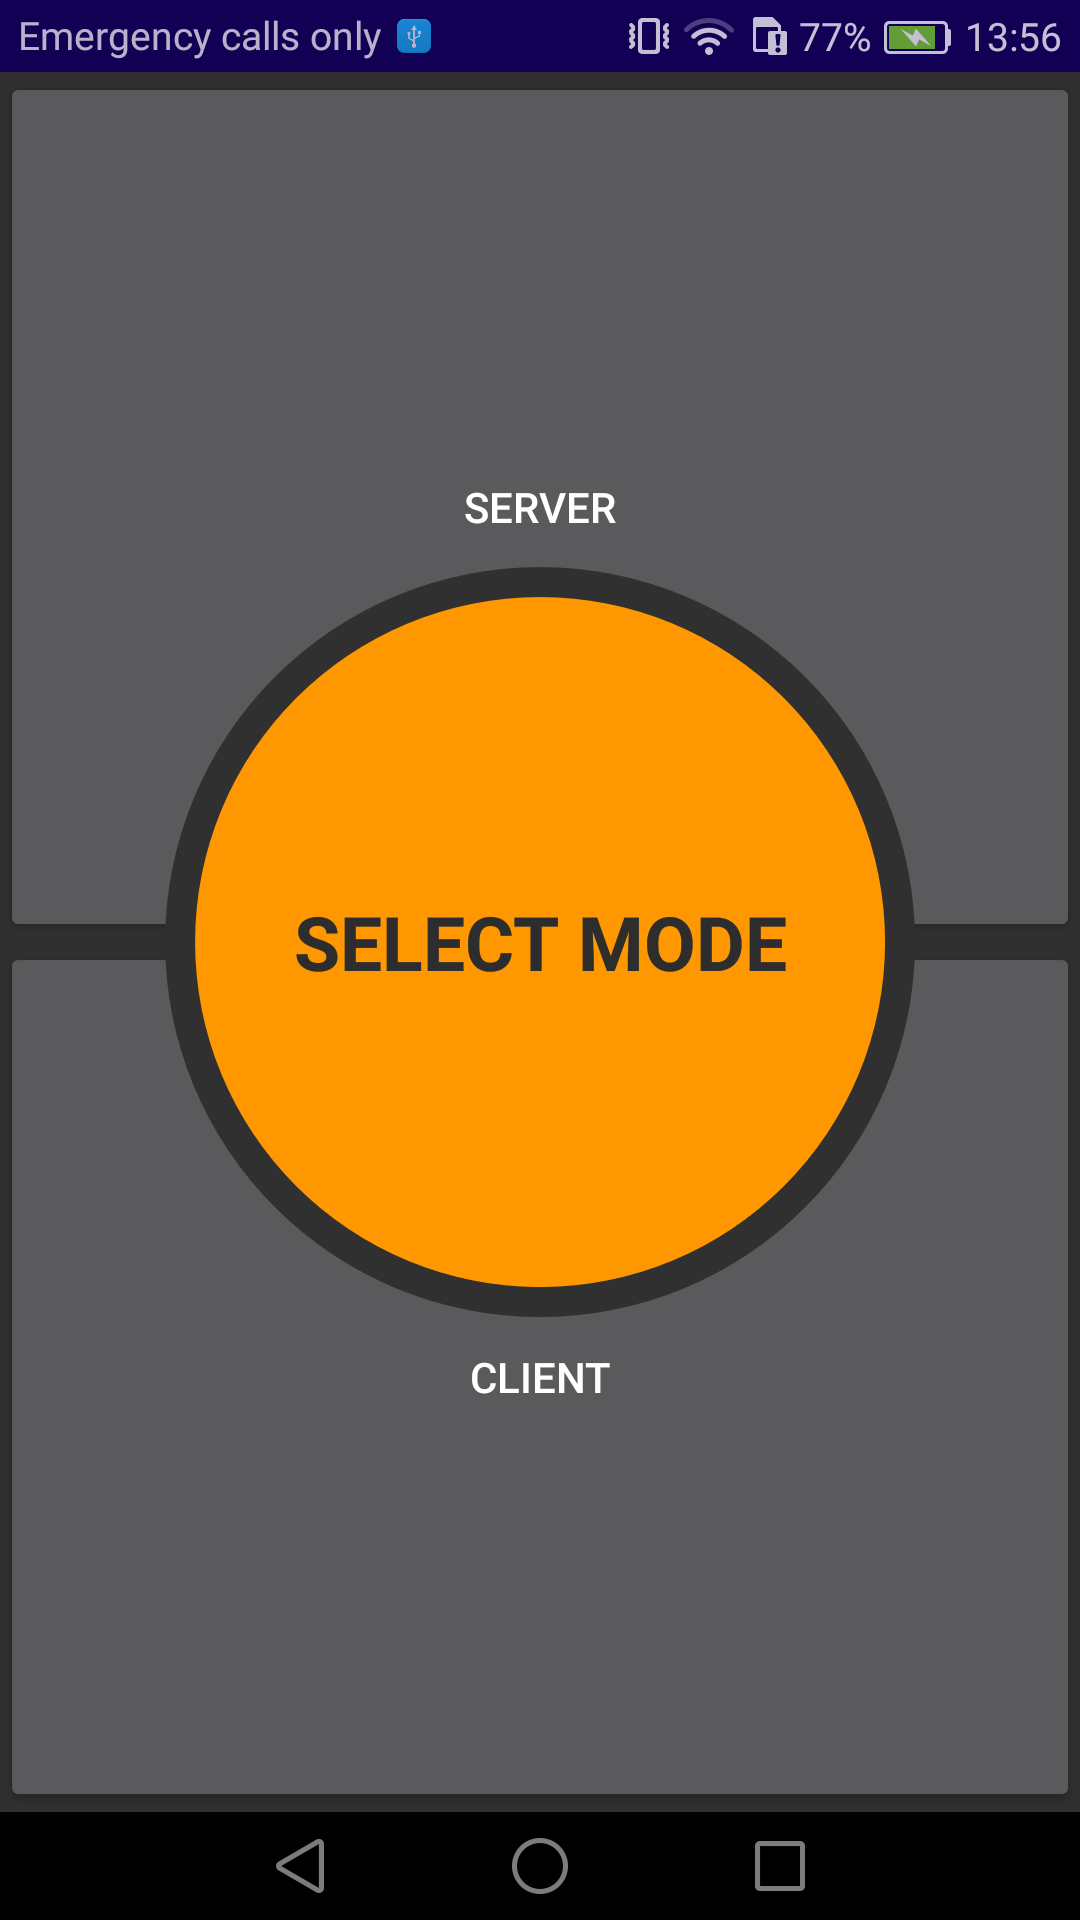
\includegraphics[trim={0cm 0cm 0cm 0cm}, clip, height=7cm]{img/ui/mode_selection.png}
    \caption{Mode Selection}
    \label{fig:mode_selection}
    \vspace{4ex}
  \end{subfigure}%%
  \begin{subfigure}[b]{0.33\linewidth}
    \centering
    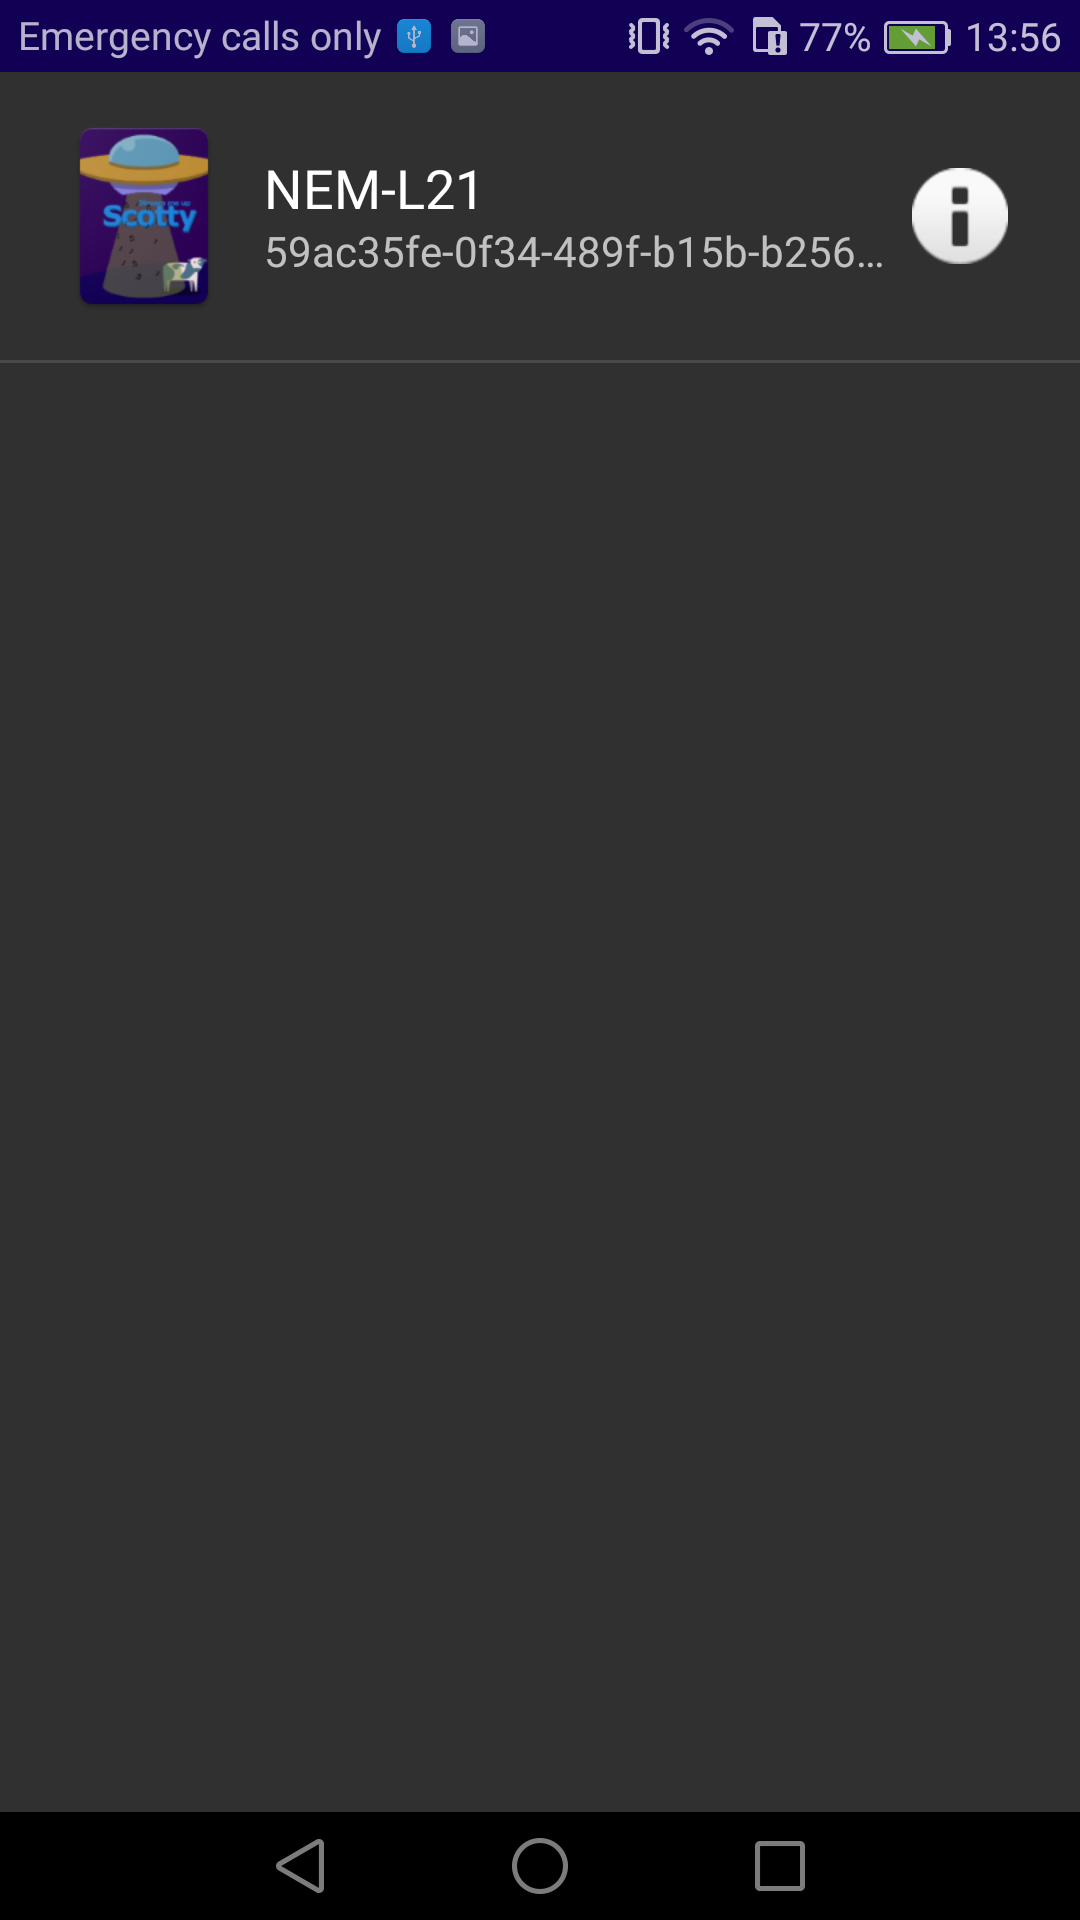
\includegraphics[trim={0cm 0cm 0cm 0cm}, clip, height=7cm]{img/ui/group_selection.png}
    \caption{Group Selection}
    \label{fig:group_selection}
    \vspace{4ex}
  \end{subfigure}%%
  \begin{subfigure}[b]{0.33\linewidth}
    \centering
    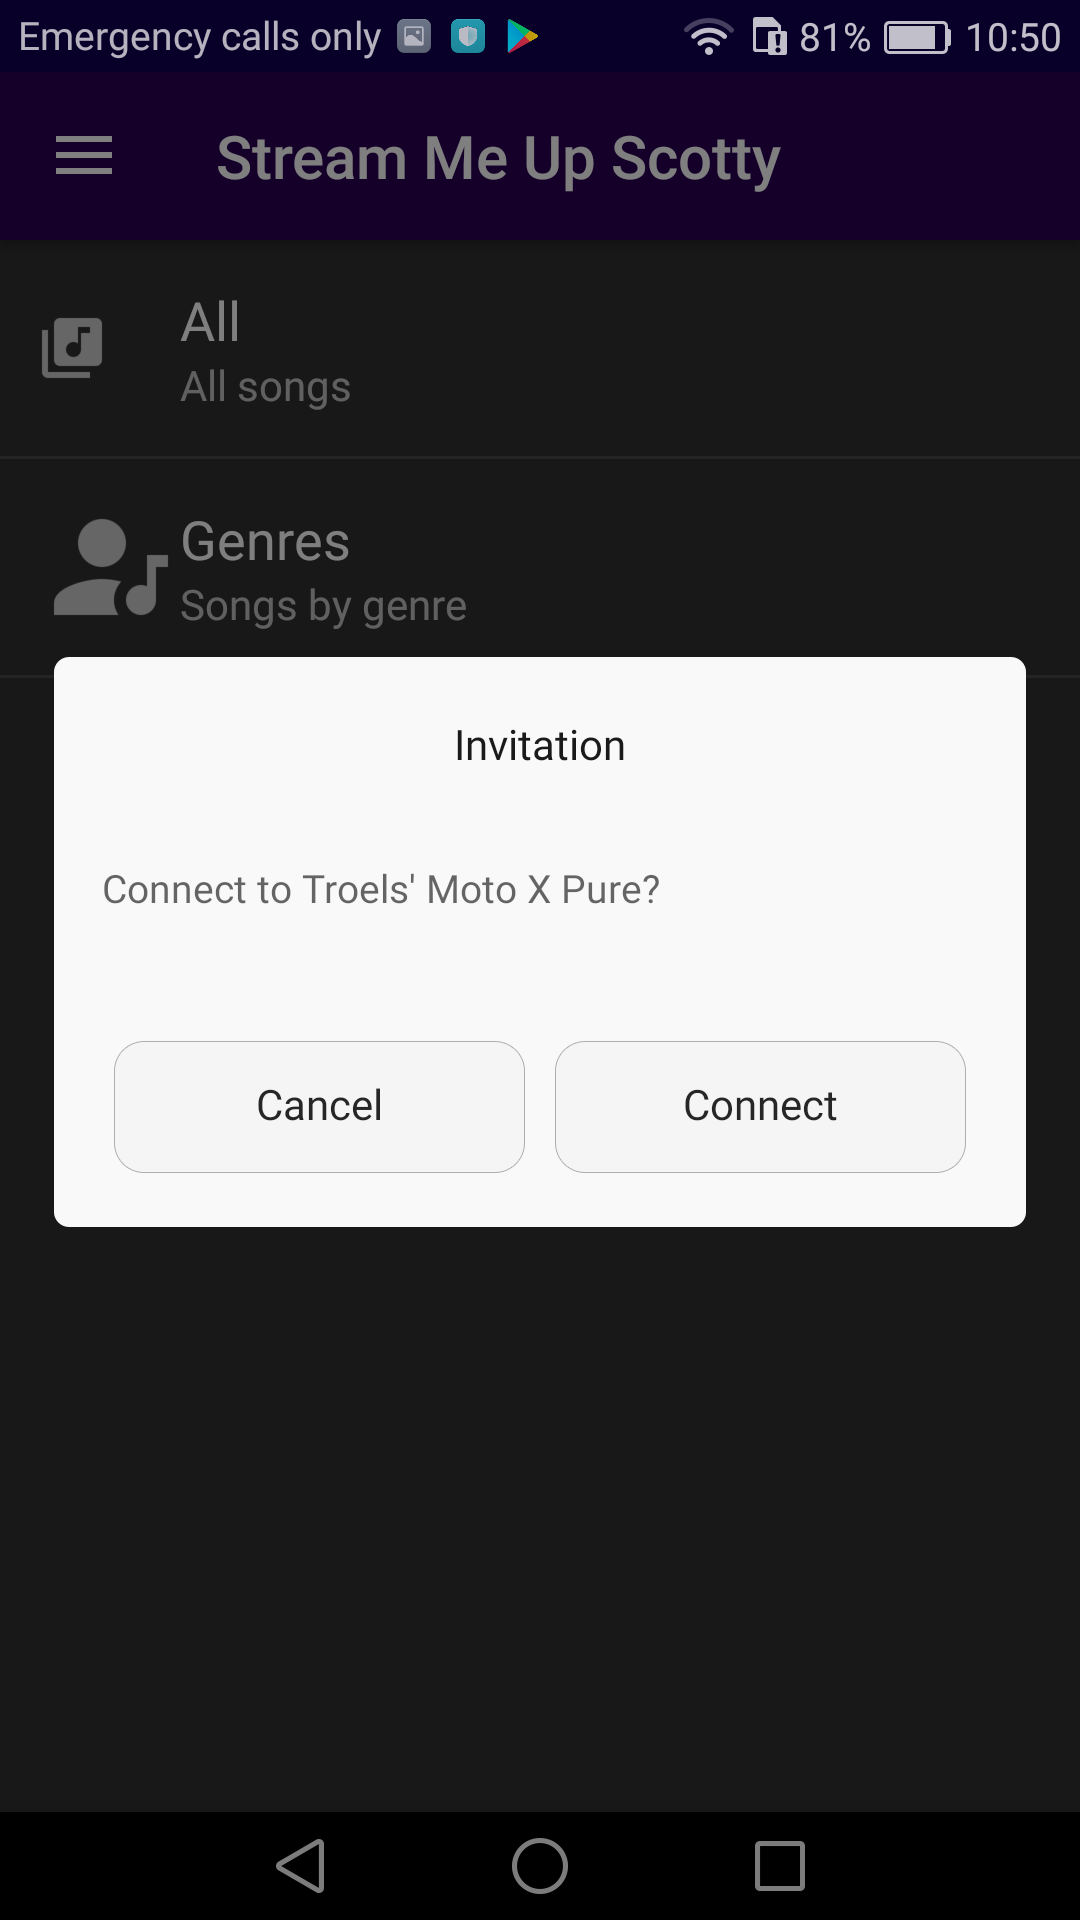
\includegraphics[trim={0cm 0cm 0cm 0cm}, clip, height=7cm]{img/ui/wifi_direct_invitation.png}
    \caption{WiFi Direct invitation}
    \label{fig:wifidirectinv}
    \vspace{4ex}
  \end{subfigure}
  \caption{The user interface relevant for connecting devices.}
  \label{fig:connecting}
\end{figure}

\subsection{Service Discovery}

The first problem which must be addressed in order to connect devices is peer discovery.
Fortunately WiFi Direct has a number of helpful services.
One of these services is ``Service Discovery'', which is made for the exact purpose of discovering peers.

In WiFi Direct, devices form groups, which has a single owner, these groups also form the basis of our sessions.
We experienced several issues implementing Service Discovery in our app, the most notable being group owner negotiation.
When devices connect using WiFi Direct, they negotiate about having the role of group owner.
The group owner is in charge of the network, and is responsible for granting new devices access etc.
For our app we want the device which is the master, to also have the role of being the group owner of the WiFi Direct network.
The root of the problem was caused by the devices keeping a record of the last 32 WiFi Direct groups which they had been a part of and who were the group owner.
This becomes a problem, when a new session is created using the same devices as a previous session, but with a different master.
For example, if a slave was the group owner, then it would be responsible for accepting new devices into the network, and not the master which is the intention.

In order to prevent this issue, we decided to erase the records of previous WiFi Direct networks, when we start discovering services.
This means that the only preexisting group, when a device connects, is the one just created by the master.
Since there is a preexisting group, then new devices will try to join it, when connecting.

We have depicted the entire service discovery as a sequence diagram on \cref{fig:seq_server_client}.
First the master starts, then it creates a group, and announces its service to the network.
Then a slave will start and discover services on the network, and present them to the user, as shown in \cref{fig:group_selection}.
The user will then decide what master to connect to.
Then the master has to approve the slave as shown in \cref{fig:wifidirectinv}.
If the slave is accepted, then they will join the network, and be sent the network info (e.g. IP of host).
\tikzexternaldisable{}
\begin{figure}[h]
    \resizebox{\linewidth}{!}{
        \begin{sequencediagram}
            \newthread{s}{Master}
            \newinst{sn}{Master Network}
            \newinst[2]{wd}{WiFi Direct}
            \newinst[2]{cn}{Slave Network}
            \newthread{c}{Slave}

            \begin{messcall}{s}{Start}{sn}{}
                \begin{messcall}{sn}{\shortstack{Announce \& \\\\Create Group}}{wd}{}
                    \begin{messcall}{c}{Start}{cn}{}
                        \begin{call}{cn}{Discover}{wd}{}
                        \end{call}
                        \begin{messcall}{cn}{Services}{c}{}
                        \end{messcall}
                        \begin{call}{c}{Connect}{cn}{Network Info}
                            \begin{call}{cn}{Join Group}{wd}{Network Info}
                                \begin{call}{wd}{Accept?}{sn}{Network Info}
                                    \begin{call}{sn}{Accept?}{s}{ACK}
                                    \end{call}
                                \end{call}
                            \end{call}
                        \end{call}
                        %\begin{messcall}{cn}{\shortstack{Establish\\\\Socket Connection}}{wd}{}
                        %    \begin{messcall}{wd}{\shortstack{Accept\\\\Socket Connection}}{sn}{}
                        %    \end{messcall}
                        %\end{messcall}
                    \end{messcall}
                \end{messcall}
            \end{messcall}
        \end{sequencediagram}
    }
    \caption{Sequence diagram, depicting how our the master announces its service and slaves connects.}\label{fig:seq_server_client}
\end{figure}
\tikzexternalenable{}
